\documentclass{article}

\usepackage[ ]{tikz}
%\usepackage[brazil]{babel}

\title{Revisão Prova 1 de Circuitos Digitais}
\author{Erickson Giesel Müller}
\date{16 de Maio de 2024}

\begin{document}
	\maketitle
	\section{Conteúdos}
		\begin{enumerate}
			\item Algebra de Boole
			\item Circuitos, Tabela-Verdade e Expressões
			\item Conversão de Expressões Booleanas (Soma de Produtos e Produtos de Soma)
			\item Simplificação Algébrica
			\item Mapas de Karnaugh
		\end{enumerate}
		
	\section{Algebra de Boole}
	
		Algebra de Boole é a matemática dos circuitos digitais, calculada usando variáveis e seus valores, é através dela que podemos demonstrar o que acontece nas portas lógicas. Uma variável pode assumir o valor 0 ou 1. Se a Variável $A$ for 1, o complemento dessa variável será 0, denominado $A$ negado ou $\overline{A}$.
		\subsection{Adição Booleana}
			É o equivalente à porta lógica $OR$. Se um dos dois termos à serem somados for 1, o resultado será 1.\\
				\hspace*{4 cm}
				\begin{tabular}{|c|c|c|}
					\hline
					A & B & A+B \\
					\hline
					0 & 0 & 0 \\
					\hline
					0 & 1 & 1 \\
					\hline
					1 & 0 & 1 \\
					\hline
					1 & 1 & 1 \\
					\hline
				\end{tabular}
				
		\subsection{Diferença entre $\overline{A}+\overline{B}$ e $\overline{A+B}$}
			\hspace*{2 cm}
			\begin{tabular}{|c|c|c|}
				\hline
				A & B & $\overline{A}+\overline{B}$ \\
				\hline
				0 & 0 & 1 \\
				\hline
				0 & 1 & 1 \\
				\hline
				1 & 0 & 1 \\
				\hline
				1 & 1 & 0 \\
				\hline
			\end{tabular}
			\hspace*{2 cm}
			\begin{tabular}{|c|c|c|}
				\hline
				A & B & $\overline{A+B}$ \\
				\hline
				0 & 0 & 1 \\
				\hline
				0 & 1 & 0 \\
				\hline
				1 & 0 & 0 \\
				\hline
				1 & 1 & 0 \\
				\hline
			\end{tabular}
			
		\subsection{Multiplicação Booleana}
			A multiplicação é equivalente à porta $AND$ e o resultado será 1 quando todas as variáveis da multiplicação forem 1. A diferença entre $\overline{A}.\overline{B}$ e $\overline{A.B}$ é que $\overline{A}.\overline{B}$ será 1 quando $A$ e $B$ forem 0, já $\overline{A.B}$ será 1 quando $A$ e $B$ forem diferentes de 1.\\
			
			\begin{tabular}{|c|c|c|}
				\hline
				A & B & $A.B$ \\
				\hline
				0 & 0 & 0 \\
				\hline
				0 & 1 & 0 \\
				\hline
				1 & 0 & 0 \\
				\hline
				1 & 1 & 1 \\
				\hline
			\end{tabular}
			\hspace*{1 cm}
			\begin{tabular}{|c|c|c|}
				\hline
				A & B & $\overline{A}.\overline{B}$ \\
				\hline
				0 & 0 & 1 \\
				\hline
				0 & 1 & 0 \\
				\hline
				1 & 0 & 0 \\
				\hline
				1 & 1 & 0 \\
				\hline
			\end{tabular}			
			\hspace*{1 cm}
			\begin{tabular}{|c|c|c|}
				\hline
				A & B & $\overline{A.B}$ \\
				\hline
				0 & 0 & 1 \\
				\hline
				0 & 1 & 1 \\
				\hline
				1 & 0 & 1 \\
				\hline
				1 & 1 & 0 \\
				\hline
			\end{tabular}
			\\
			Podemos perceber que $\overline{A}+\overline{B}$ é igual a $\overline{A.B}$; e $\overline{A+B}$ é igual a $\overline{A}.\overline{B}$. Teorema de DeMorgan.
	\section{Mapa de Karnaugh}		
		O mapa de Karnaugh é muito utilizado em questões em que o professor pede para montar um circuito de acordo com tais requisitos, como por exemplo:\\
		\begin{enumerate}
			\item Monte um circuito em que a saída S tem sinal de \textbf{nível lógico ALTO} quando A é 0 e B e C são iguais
		\end{enumerate}
		Nesse caso, o circuito que iremos montar tem 3 variáveis, portanto vamos fazer um mapa de Karnaugh 2x4, de 8 minitermos:\\
		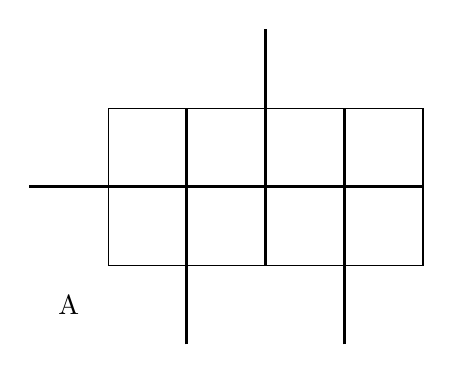
\begin{tikzpicture}
			\draw [very thick](0,2) -- (5,2);
			\draw[very thick](	2,0) -- (2,3);
			\draw[very thick](3,1) -- (3,4);
			\draw[very thick](4,0) -- (4,3);
			\draw[step=1 cm] (1,1) grid (5,3);
			
			\draw (.5,.5) node{A};
		\end{tikzpicture}
\end{document}